The objective function in Eq. \ref{rec1} can be optimized using different techniques. Earlier approaches
\citep{carr00,cap04} solve the problem using only branch-and-bound technique \citep{past82,bets97} or branch-and-cut technique the latter of which can be considered as an \emph{integer constrained relaxation} method for integer programming \citep{mitc98}. However, as suggested in the optimization literature \citep{bert99,bets97}, significant computation advantage can be gained by performing \emph{Lagrangian relaxation} as well. In such relaxation, first a feasible set is formulated where the \emph{Lagrangian} is optimized \emph{w.r.t} the \emph{primal variables} and the dual objective is optimized thereafter yielding a lower (for minimization) or upper bound (for maximization) to the original objective. The duality gap can further be improved by proposing better constraint sets \citep{bert99,bets97}. Additionally, in case of a non-zero duality gap, one can employ branch-and-bound algorithm on the smaller feasible set obtained from the Lagrangian relaxation. In this section, first a tighter constrain set, proposed by \citet{anmy11}, is presented which is then followed by the Lagrangian relaxation and an application of the branch-and-bound algorithm.

\subsection{Finding a Tighter Constrain Set}

Tightening the solution space may improve the bound of the proposed Lagrangian \citep{ackm05,bert99}. To increase the constrain set for a tighter relaxation, the constraint \ref{rec3} and \ref{rec5} are replaced by the following two constraints:
\begin{equation}
\label{rec8}
x_{ik}  \geq \sum\limits_{(r,s) \in row _{ik}(j)}  y_{rsik} ,	    j\in {\delta _1^+(i)}, i \in [1,n_1] , k \in [1,n_2]
\end{equation}
\begin{equation}
\label{rec9}
x_{ik}  \geq \sum\limits_{(r,s) \in col _{ik} (l)}  y_{ikjl} ,	    l\in {\delta _2^-(k)}, i \in [2,n_1] , k \in [2,n_2]
\end{equation}
The construction of $row _{ik}(j)$ and $col _{ik} (l)$ in Eqs. \ref{rec8} and \ref{rec9} can be explained with the Fig. \ref{fig:Construction of tighter constraint set}. The grey area in each of the images is the rectangle formed by $\delta_1^-(i)$ rows and $\delta_2^-(k)$ colums for any vertex (i,k) in the graph. Let $(i_1,i_2,\cdots,i_s)$ and $(k_1,k_2,\cdots,k_t)$ be the ordered set of vertices in $\delta_1^-(i)$ and $\delta_2^-(k)$. Considering the vertices in the $l^{\text{th}}$ column to be the pairwise crossing matching, at most one of the points in the vertices of the column will satisfy Eq. \ref{rec5}. The solution remains the same even if the following sets are added to the vertices in the $l^{\text{th}}$ column:$(i_s,k_1),(i_s,k_2),\cdots,(i_s,k_{l-1})$ and $(i_1,k_{l+1},i_1,k_{l+2},\cdots,i_1,k_t)$. The union of these three sets constructs $col _{ik} (l)$. $row _{ik}(j)$ is constructed in a similar fashion.

\begin{figure}[ht]
\centering
 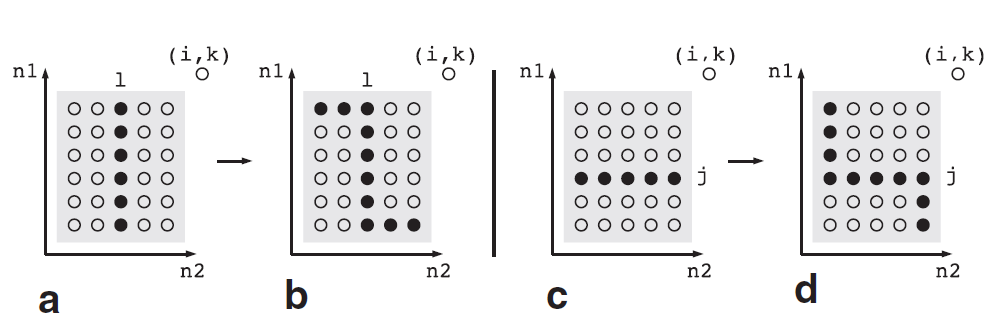
\includegraphics[width=0.7\textwidth]{pic2}
 \caption{Construction of tighter constraint set}
 \label{fig:Construction of tighter constraint set}
\end{figure}

\subsection{Lagrangian Relaxation}
The Lagrangian of the problem in Eq. \ref{rec1} is formed as follows:
\begin{equation}
\label{lagrangian}
\mathcal{L}(\mathbf{x},\mathbf{y},\boldsymbol{\lambda}) = \sum\limits_{(ik)(jl) \in E^{\prime}} y_{ikjl}
+ \displaystyle\sum_{i,k,j\in\delta_{1}^{-1}(i)}\lambda_{ikj}^{h} \left(x_{ik} - \displaystyle\sum_{(r,s)\in\text{row}_{ik}(j)}y_{rsik}\right)
\end{equation}
\begin{equation}
+ \displaystyle\sum_{i,k,l\in\delta_{2}^{-1}(k)}\lambda_{ikl}^{v} \left(x_{ik} - \displaystyle\sum_{(r,s)\in\text{col}_{ik}(j)}y_{rsik}\right)
\end{equation}
with the constraints \ref{rec2},\ref{rec4},\ref{rec6},\ref{rec7} and $\boldsymbol{\lambda} = \{\{\lambda_{ikj}^{h}\}, \{\lambda_{ikl}^{v}\}\}\ge \mathbf{0}$. The maximization over the primal variables
$\mathbf{x},\mathbf{y}$ can be performed in $O(|V^{\prime}|+|E^{\prime}|)$ time and this becomes obvious if the objective in Eq. \ref{lagrangian} is observed more carefully. One can see that the objective decomposes over the primal variables and essentially there are as many subproblems as there are number of primal variables in the objective, each of which can be solved independently. Moreover, two different sets of sub-problems can be defined. The first one corresponds to finding the set of best \emph{local variable} $y_{ijkl}$ pertaining to each vertex $(i,k)\in V^{\prime}$ that respects the constrains. The second one corresponds to finding the best values of the set of \emph{global variables} $\{x_{ik}\}$'s. Simple dynamic programming based computation shows a run time complexity of
$O(|V^{\prime}|+|E^{\prime}|)$.

\begin{figure}[htbp]
\centering
 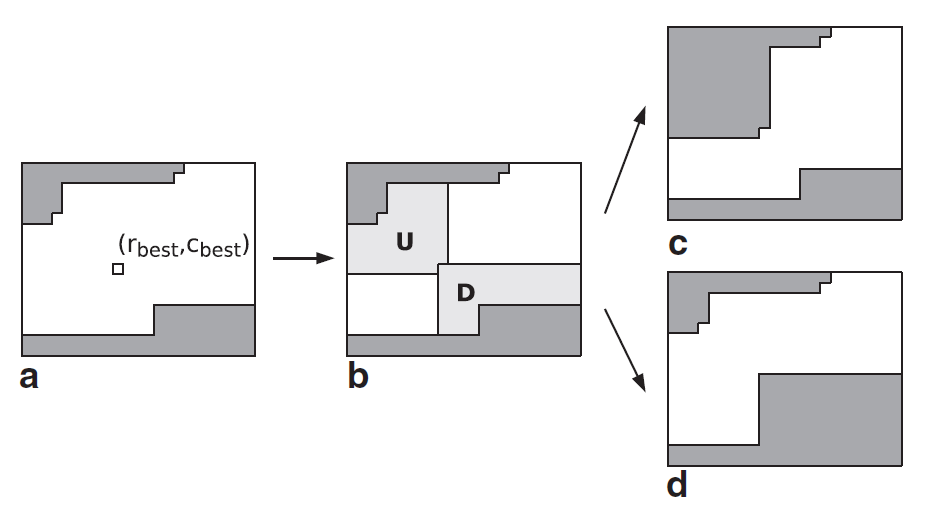
\includegraphics[width=0.7\textwidth]{pic3}
 \caption{Branch-and-bound Splitting Strategy}
 \label{fig:BB}
\end{figure}

A dual objective function $\mu(\boldsymbol{\lambda})$ is obtained afterwards
by maximizing \ref{lagrangian} over the primal variables. The dual objective, however, has plenty of variables $\boldsymbol{\lambda}$ and hence sub-gradient descent \citep{hewc74,duhs11} with adaptive step-size regulation is used. However, the bound so obtained is not tight and there might exist duality gap either because of problem formulation or from the approximations used in the sub-gradient optimization. To make the solution even better, branch-and-bound algorithm is used as discussed in the next section.

\subsection{Branch-and-bound Algorithm}

A branch-and-bound algorithm works by enumerating over all possible solution sets and maintaining a tree structure to prune the search space based on the value of the objective function. Parts of the tree where the objective function takes bigger value (in case of maximization), are preferred over other parts of the tree.
A node in the tree in the current setting is given by by $n_2$ couples $(b_k, t_k)$ for $k_2 \in [1, n2]$ which define the candidate vertex set $Cand$ (the white area in-between the two broken lines on Fig. \ref{fig:BB}).
A vertex $(j, l)$ of the graph $B^{\prime}$ belongs to $Cand$ if $b_l\leq j \leq t_l$.
For any vertex $(j,l) \in Cand$, two sets are created:
$U(j,l)= \{(i, k) \in Cand : (i, k)=(j, l), i\ge j, k\le l\}$
and $D(j,l) = f(i, k) \in Cand : i\le j, k\ge l\}$.
By definition, if a feasible path has a vertex in $U(j,l)$, it cannot
have one in $D(j,l)$, and \emph{vice versa}.
Let $(rbest, cbest)$ be the $\arg\max_{(j, l)\in Cand} \min (\|D(j, l)\|, \|U(j, l)\|)$. Now, the two descendants of the current node are obtained by discarding from its feasible set the vertices belonging to the two respective domains $U(rbest,cbest)$ and $D(rbest, cbest)$ (refer to Fig. \ref{fig:BB}). The goal of this strategy is twofold: to create descendants that are balanced in sense of feasible set size and to reduce maximally the parent node’s feasible set. 